% ============================================================
%  methods_draft.tex
%  A STANDALONE rough AI draft (Introduction through Conclusion) — NOT the
%  manuscript. Kept separate from main.tex so it can be revised freely.
%  Intro/Background prose is adapted and expanded from main.tex.
%
%  It pulls in the auto-generated assets written by
%  scripts/export_paper_assets.py:
%    - figures from  generated/figures/   (white-background PDFs)
%    - tables  from  generated/tables/
%    - numbers from  generated/stats.tex  (macros like \statOverlapMean)
%
%  Compile from inside manuscript/ so the relative paths resolve:
%    pdflatex methods_draft -> bibtex methods_draft -> pdflatex methods_draft x2
% ============================================================
\documentclass[12pt,a4paper]{article}

% ---- Match the manuscript's look ----
\usepackage[T1]{fontenc}
\usepackage[utf8]{inputenc}
\usepackage{newtxtext,newtxmath}            % Times New Roman-like text + math
\usepackage[a4paper,left=2cm,right=2cm,top=2cm,bottom=2cm]{geometry}
\usepackage{setspace}\onehalfspacing
\usepackage{microtype}
\usepackage{amsmath}
\usepackage{graphicx}
\usepackage{booktabs}                        % the generated tables use \toprule etc.
\usepackage[round,authoryear]{natbib}
\usepackage[hidelinks]{hyperref}

% ---- Where to find the generated assets ----
\graphicspath{{generated/figures/}}
% Auto-generated by scripts/export_paper_assets.py — do not edit by hand.
% Each macro is a number quoted in the manuscript; re-run the script to refresh.
% Usage in main.tex:  % Auto-generated by scripts/export_paper_assets.py — do not edit by hand.
% Each macro is a number quoted in the manuscript; re-run the script to refresh.
% Usage in main.tex:  % Auto-generated by scripts/export_paper_assets.py — do not edit by hand.
% Each macro is a number quoted in the manuscript; re-run the script to refresh.
% Usage in main.tex:  \input{generated/stats.tex}   then e.g.  \statOverlapMean

\newcommand{\statNCitiesAnalyzed}{387}
\newcommand{\statOverlapMean}{0.946}
\newcommand{\statOverlapMedian}{0.960}
\newcommand{\statOverlapSkew}{-1.33}
\newcommand{\statOverlapKurt}{1.46}
\newcommand{\statSizePapersR}{+0.71}
\newcommand{\statSizePapersP}{0.000}
\newcommand{\statSizeProjectsR}{+0.70}
\newcommand{\statSizeProjectsP}{0.000}
\newcommand{\statClusterNCitiesAll}{323}
\newcommand{\statClusterMinDocs}{8}
\newcommand{\statClusterNCitiesDense}{60}
\newcommand{\statClusterOlsRsq}{0.064}
\newcommand{\statClusterSizePapersP}{0.066}
\newcommand{\statClusterSizeProjectsP}{0.539}
\newcommand{\statClusterPermObserved}{0.0590}
\newcommand{\statClusterPermNullMean}{0.0390}
\newcommand{\statClusterPermP}{0.0005}
\newcommand{\statClusterPermExcess}{+0.0200}
\newcommand{\statMantelR}{+0.21}
\newcommand{\statMantelP}{0.0010}
\newcommand{\statMantelNCities}{244}
\newcommand{\statNPapersTotal}{10,319}
\newcommand{\statNProjectsTotal}{4,606}
\newcommand{\statPaperYearMin}{2000}
\newcommand{\statPaperYearMax}{2026}
\newcommand{\statProjectYearMin}{2009}
\newcommand{\statProjectYearMax}{2025}
\newcommand{\statAlignMeanDelta}{+0.0135}
\newcommand{\statAlignFracPos}{0.908}
\newcommand{\statAlignT}{77.99}
\newcommand{\statAlignP}{0.0000}
\newcommand{\statAlignNProjects}{3,596}
\newcommand{\statAlignTClustered}{17.70}
\newcommand{\statAlignNCities}{320}
\newcommand{\statAlignDeltaCity}{+0.0084}
\newcommand{\statAlignTCity}{12.19}
\newcommand{\statAlignFracCitiesPos}{0.791}
\newcommand{\statAlignSizeR}{+0.59}
\newcommand{\statAlignSizeP}{0.000}
\newcommand{\statAlignDeltaLarge}{+0.0165}
\newcommand{\statAlignDeltaSmall}{+0.0045}
\newcommand{\statCcAlignN}{111}
\newcommand{\statCcAlignNCities}{79}
\newcommand{\statCcAlignMeanDelta}{+0.0140}
\newcommand{\statCcAlignFracPos}{0.901}
\newcommand{\statCcAlignTClustered}{9.50}
\newcommand{\statDidEstimate}{+0.0026}
\newcommand{\statDidT}{7.33}
\newcommand{\statDidP}{0.0000}
\newcommand{\statDidN}{1,834}
\newcommand{\statDidTClustered}{4.06}
\newcommand{\statDidNCities}{161}
\newcommand{\statLeadlagBestLag}{+3}
\newcommand{\statLeadlagBestSim}{0.9003}
\newcommand{\statNCitiesParts}{348}
\newcommand{\statPartEntropyMedian}{1.557}
\newcommand{\statPartEntropyMax}{3.584}
   then e.g.  \statOverlapMean

\newcommand{\statNCitiesAnalyzed}{387}
\newcommand{\statOverlapMean}{0.946}
\newcommand{\statOverlapMedian}{0.960}
\newcommand{\statOverlapSkew}{-1.33}
\newcommand{\statOverlapKurt}{1.46}
\newcommand{\statSizePapersR}{+0.71}
\newcommand{\statSizePapersP}{0.000}
\newcommand{\statSizeProjectsR}{+0.70}
\newcommand{\statSizeProjectsP}{0.000}
\newcommand{\statClusterNCitiesAll}{323}
\newcommand{\statClusterMinDocs}{8}
\newcommand{\statClusterNCitiesDense}{60}
\newcommand{\statClusterOlsRsq}{0.064}
\newcommand{\statClusterSizePapersP}{0.066}
\newcommand{\statClusterSizeProjectsP}{0.539}
\newcommand{\statClusterPermObserved}{0.0590}
\newcommand{\statClusterPermNullMean}{0.0390}
\newcommand{\statClusterPermP}{0.0005}
\newcommand{\statClusterPermExcess}{+0.0200}
\newcommand{\statMantelR}{+0.21}
\newcommand{\statMantelP}{0.0010}
\newcommand{\statMantelNCities}{244}
\newcommand{\statNPapersTotal}{10,319}
\newcommand{\statNProjectsTotal}{4,606}
\newcommand{\statPaperYearMin}{2000}
\newcommand{\statPaperYearMax}{2026}
\newcommand{\statProjectYearMin}{2009}
\newcommand{\statProjectYearMax}{2025}
\newcommand{\statAlignMeanDelta}{+0.0135}
\newcommand{\statAlignFracPos}{0.908}
\newcommand{\statAlignT}{77.99}
\newcommand{\statAlignP}{0.0000}
\newcommand{\statAlignNProjects}{3,596}
\newcommand{\statAlignTClustered}{17.70}
\newcommand{\statAlignNCities}{320}
\newcommand{\statAlignDeltaCity}{+0.0084}
\newcommand{\statAlignTCity}{12.19}
\newcommand{\statAlignFracCitiesPos}{0.791}
\newcommand{\statAlignSizeR}{+0.59}
\newcommand{\statAlignSizeP}{0.000}
\newcommand{\statAlignDeltaLarge}{+0.0165}
\newcommand{\statAlignDeltaSmall}{+0.0045}
\newcommand{\statCcAlignN}{111}
\newcommand{\statCcAlignNCities}{79}
\newcommand{\statCcAlignMeanDelta}{+0.0140}
\newcommand{\statCcAlignFracPos}{0.901}
\newcommand{\statCcAlignTClustered}{9.50}
\newcommand{\statDidEstimate}{+0.0026}
\newcommand{\statDidT}{7.33}
\newcommand{\statDidP}{0.0000}
\newcommand{\statDidN}{1,834}
\newcommand{\statDidTClustered}{4.06}
\newcommand{\statDidNCities}{161}
\newcommand{\statLeadlagBestLag}{+3}
\newcommand{\statLeadlagBestSim}{0.9003}
\newcommand{\statNCitiesParts}{348}
\newcommand{\statPartEntropyMedian}{1.557}
\newcommand{\statPartEntropyMax}{3.584}
   then e.g.  \statOverlapMean

\newcommand{\statNCitiesAnalyzed}{387}
\newcommand{\statOverlapMean}{0.946}
\newcommand{\statOverlapMedian}{0.960}
\newcommand{\statOverlapSkew}{-1.33}
\newcommand{\statOverlapKurt}{1.46}
\newcommand{\statSizePapersR}{+0.71}
\newcommand{\statSizePapersP}{0.000}
\newcommand{\statSizeProjectsR}{+0.70}
\newcommand{\statSizeProjectsP}{0.000}
\newcommand{\statClusterNCitiesAll}{323}
\newcommand{\statClusterMinDocs}{8}
\newcommand{\statClusterNCitiesDense}{60}
\newcommand{\statClusterOlsRsq}{0.064}
\newcommand{\statClusterSizePapersP}{0.066}
\newcommand{\statClusterSizeProjectsP}{0.539}
\newcommand{\statClusterPermObserved}{0.0590}
\newcommand{\statClusterPermNullMean}{0.0390}
\newcommand{\statClusterPermP}{0.0005}
\newcommand{\statClusterPermExcess}{+0.0200}
\newcommand{\statMantelR}{+0.21}
\newcommand{\statMantelP}{0.0010}
\newcommand{\statMantelNCities}{244}
\newcommand{\statNPapersTotal}{10,319}
\newcommand{\statNProjectsTotal}{4,606}
\newcommand{\statPaperYearMin}{2000}
\newcommand{\statPaperYearMax}{2026}
\newcommand{\statProjectYearMin}{2009}
\newcommand{\statProjectYearMax}{2025}
\newcommand{\statAlignMeanDelta}{+0.0135}
\newcommand{\statAlignFracPos}{0.908}
\newcommand{\statAlignT}{77.99}
\newcommand{\statAlignP}{0.0000}
\newcommand{\statAlignNProjects}{3,596}
\newcommand{\statAlignTClustered}{17.70}
\newcommand{\statAlignNCities}{320}
\newcommand{\statAlignDeltaCity}{+0.0084}
\newcommand{\statAlignTCity}{12.19}
\newcommand{\statAlignFracCitiesPos}{0.791}
\newcommand{\statAlignSizeR}{+0.59}
\newcommand{\statAlignSizeP}{0.000}
\newcommand{\statAlignDeltaLarge}{+0.0165}
\newcommand{\statAlignDeltaSmall}{+0.0045}
\newcommand{\statCcAlignN}{111}
\newcommand{\statCcAlignNCities}{79}
\newcommand{\statCcAlignMeanDelta}{+0.0140}
\newcommand{\statCcAlignFracPos}{0.901}
\newcommand{\statCcAlignTClustered}{9.50}
\newcommand{\statDidEstimate}{+0.0026}
\newcommand{\statDidT}{7.33}
\newcommand{\statDidP}{0.0000}
\newcommand{\statDidN}{1,834}
\newcommand{\statDidTClustered}{4.06}
\newcommand{\statDidNCities}{161}
\newcommand{\statLeadlagBestLag}{+3}
\newcommand{\statLeadlagBestSim}{0.9003}
\newcommand{\statNCitiesParts}{348}
\newcommand{\statPartEntropyMedian}{1.557}
\newcommand{\statPartEntropyMax}{3.584}
                  % defines \statOverlapMean, \statNCitiesAnalyzed, ...

\title{Patents, Papers, Parts, and Planet\\[0.4em]{\large\itshape Rough AI Draft}}
\date{}

\begin{document}
\maketitle

\begin{center}
\fbox{\parbox{0.92\linewidth}{\centering\small\itshape
This is a rough, AI-assisted working draft. Prose, structure, and emphasis are
provisional and under active revision; numbers and figures are generated from
the analysis pipeline but the surrounding argument has not yet been finalised.}}
\end{center}
\vspace{1em}

% ============================================================
\section{Introduction}
% ============================================================

% --- Research question -------------------------------------------------------
\subsection{Research question}

This thesis asks a single question: \textbf{do cities with student synthetic
biology research also produce academic papers in related areas?} Put more
carefully: when a city's iGEM teams take up a theme, do that city's researchers
publish on related themes, and can we see the relatedness in the text both groups
leave behind? The chapters that follow build the data and the measures to answer
it, then test that answer to breaking point. Throughout, we speak of
\textit{semantic relatedness} and \textit{co-location}, and we avoid the language
of cause and effect.

\subsection{Synthetic Biology}

Humanity has always sought to understand and influence the natural world. Biology,
the study of life itself, spent most of its history describing it, breaking
organisms into their parts to work out the principles that hold them together.
That descriptive work gave rise to something new. Once we understood life's
principles well enough, we began to \textit{write} with them, designing and
directing new biological systems of our own. This is the age of Synthetic Biology:
a field that treats genetic sequences as functions in the programming language of
life, standardises them, and snaps them together into genetic circuits
\citep{wayIntegratingBiologicalRedesign2014}. A living cell becomes a kind of
programmable factory. A single sequence might switch a gene on, report a signal,
or drive a metabolic pathway. The parts compose much like software, and the living
machinery that results is a tool we can aim at problems of our own choosing.

That shift from describing life to engineering it is recent, and it is moving
fast. In a couple of decades Synthetic Biology has grown from a handful of
proof-of-concept circuits into a field with real stakes in medicine, materials,
agriculture, and energy
\citep{shapiraTrackingEmergenceSynthetic2017, raimbaultMappingEmergenceSynthetic2016}.
It is also hard to pin down. Its boundaries keep moving, and its vocabulary
overlaps heavily with the descriptive molecular biology it grew out of. A young
field this consequential is worth watching closely, and worth asking where its
innovation happens and who is doing it.

\subsection{iGEM}

One arena where that innovation takes shape early is iGEM. The International
Genetically Engineered Machine competition is a worldwide student contest in
Synthetic Biology, a sort of LEGO-robotics contest for genetic engineering. Teams
of students, usually hosted by a university, spend most of a year designing and
building an original project with the tools of the field. Every team starts from
the same kit of standardised parts and the same basic rules, then is left to
invent its own entry. They document that entry in public on a project ``wiki'', a
page that reads much like an extended research abstract
\citep{santoliniIGEMModelSystem2023}.

iGEM matters here for more than its scale. For many researchers it is a first
serious project in Synthetic Biology, and a launching point for a career in
academia or industry. Its alumni have founded companies and started labs of their
own. iGEM styles itself as ``the heart of synthetic biology,'' and it isn't only
hype. The competition also sets norms that reach well beyond it: open science,
thorough public documentation, and a shared registry of standardised,
interoperable parts. Those norms are what make iGEM legible to a study like this
one. Thousands of projects, each documented the same way and each tied to a place
and a year, add up to a detailed record of a field as it grows.

% --- Argument and central claim ---------------------------------------------
\subsection{From iGEM to a testable claim}

That record is what makes iGEM worth studying, because it sits near the base of a
larger chain. Innovation rests on research: new products grow out of people
investigating what is possible. Synthetic Biology is one of the most active
frontiers of that work, and iGEM is where a large share of its practitioners first
learn to do it. If we want to know how innovation in the field takes root, and how
its ideas travel, the student projects at the entry point are a natural place to
start.

This thesis makes one central, testable claim. When a city's student teams take up
a theme, say biosensors or carbon capture, that city's published papers should
concentrate in related areas, more than they would in a city that produced the
same amount of work on unrelated themes. The claim is about \textit{relatedness}:
whether student and academic work sit in the same corners of the field in the same
places. It is not a claim about cause. Everything that follows is built to state
it precisely, then try hard to knock it down.

% --- The artifacts -----------------------------------------------------------
\subsection{Reading capabilities off artifacts}

Capabilities are abstract, so we read them off the concrete things a place
produces. Each kind of artifact records the creation of new knowledge in its own
way, while pointing back to the same underlying capability. An academic paper is
the currency of scholarship, rewarded by its influence on a field. A patent is a
claim on commercial value, filed because someone expects an idea to pay. The two
often diverge. A landmark result can have no obvious market, and a lucrative
patent can hold little that is scientifically new. Synthetic Biology adds a third
kind of record that few fields keep so openly: the student project, published in
full by teams still learning the craft. Different as these artifacts are in
audience and incentive, they grow out of the same local pool of people and
equipment, which is why comparing them can tell us something about a place.

This thesis works with four such artifacts, though unevenly. Its spine is the
pairing of student \textit{projects} with academic \textit{papers}, the two we can
line up most directly. The physical \textit{parts} that teams register,
standardised fragments of DNA, give a text-independent check on whether the story
the text tells holds up. \textit{Patents}, the bridge from research to commercial
application and one of the P's the project is named for, are set up here but left
largely to future work, for practical reasons the Conclusion makes concrete.
Table~\ref{tab:artifacts} summarises what each artifact is and the role it plays.
A reader should leave this section knowing which promises the Results pay off, and
which are still roadmap.

\begin{table}[htbp]
  \centering
  \small
  \begin{tabular}{@{}l p{3.3cm} p{4.1cm} p{3.6cm}@{}}
    \toprule
    Artifact & What it is & What it signals & Role in this thesis \\
    \midrule
    iGEM projects & Year-long student projects, documented on public wikis &
      Where new practitioners take up themes & Primary (paired with papers) \\
    Academic papers & Peer-reviewed publications (from OpenAlex) &
      Scholarly work and its impact on a field & Primary (paired with projects) \\
    BioBrick parts & Standardised DNA fragments teams register &
      What a city's teams physically built & Corroboration (independent of text) \\
    Patents & Filings claiming commercial rights &
      Belief in an idea's commercial value & Motivated; left to future work \\
    \bottomrule
  \end{tabular}
  \caption{The four artifact types this thesis considers, what each one records,
  and the role it plays in the analysis. Projects and papers are the primary
  pairing; parts corroborate the text from outside it; patents are set up but
  deferred.}
  \label{tab:artifacts}
\end{table}

% --- The ``Planet'' lens ------------------------------------------------------
\subsection{The ``Planet'' lens: carbon capture}

The modern industrial era reshaped the planet. We burned through vast reserves of
ancient carbon, and in doing so we lived longer, fed more people, and grew past
every earlier limit. We also changed the climate. The change is large enough that
scientists have proposed a new geological epoch to mark it, the Anthropocene
\citep{crutzen2006anthropocene}, an age in which human activity is a dominant
force on the Earth system. We are terraforming our own planet, mostly by accident.

There is a hopeful reading of that same fact. If we can knock a planet's climate
off balance without trying, then the same power, aimed on purpose, might help set
it right. Biology is one of the best tools for the job, and carbon capture is
where this thesis watches it work. Humanity's oldest biotechnology is control over
fermentation: we brewed and baked with microbes long before we could name one.
Synthetic Biology turns that old craft to a new end, engineering microbes such as
\textit{E.\,coli} to pull carbon from industrial exhaust and build it into fuels
and materials \citep{delisiRoleSyntheticBiology2020, gleizerConversionEscherichiaColi2019}.

Carbon capture runs through the whole project as a single thread. It's concrete,
and we can trace it from a student's bench to a patent filing. We tag projects,
papers, and parts for their relevance to it, and follow the theme across all of
them. Late in the analysis it does a second job. Every artifact we study is
already synthetic biology, so any two of them look somewhat alike. Narrowing to
one sub-topic strips that shared baseline away, so we can ask whether local
relatedness still holds inside it.

% --- Unit of analysis --------------------------------------------------------
\subsection{Why cities?}

Innovation in synthetic biology is not spread evenly across the map. It clusters,
and it clusters in cities. The reasons pile up in the same places: universities
with expensive equipment and talented students, venture capital for startups,
established industries like pharma that already own the infrastructure, and
regulators willing to permit the work. Deep-tech research needs all of these at
once, and cities are where they coincide.

Cities also specialise. Regions build capability in particular technologies, then
branch into adjacent ones over time \citep{hidalgoProductSpaceConditions2007}, so
different cities should develop different strengths \emph{within} synthetic
biology. A city with a strong software sector may build better computational
tools. One with deep agricultural roots may scale engineered crops more easily.
Where a research university dominates, the local edge may be foundational science
instead. This is the structure the thesis is after, and the reason the city is our
unit.

To read a city's strengths we pool its documents instead of judging them one at a
time. A single project or paper is a noisy signal, shaped as much by one team's
quirks as by the place around it. Pooled together, a city's output settles into
something steadier: a coarse-grained picture of what that place works on. We
aggregate across years as well, treating each city as one accumulated body of
work, since most cities produce too little in any single year to characterise on
their own. What we compare, in the end, is one city's body of work against
another's.

% --- Worked example ----------------------------------------------------------
\subsection{A worked example}

The case study is where this stops being abstract. Near the end we pick one
carbon-capture project and follow its threads outward: the BioBricks it
registered, the papers those parts were built from, the later papers that cite
them, and the patents that carry the same sequences. One project, traced through
every artifact type at once, shows in miniature the local trajectory the rest of
the thesis can only measure in aggregate.

% --- Scope and contributions -------------------------------------------------
\subsection{Scope and contributions}

A caution belongs here, at the front. This thesis shows relatedness. It does not
show causation. When a city's projects and papers sit close in meaning, many
shared causes could put them there: the same university, the same funding, the
same handful of advisors who mentor students by day and publish by night. We
cannot separate a real flow of ideas from a lab that simply houses both kinds of
work, and we do not try to. Every result that follows is a statement about
association and co-location, and we say so plainly wherever it matters.

The thesis makes four contributions, all concrete. The first is a corpus that puts
iGEM projects, academic papers, and BioBrick parts under one shared schema, each
geocoded to a city. The second is an embedding-based measure of how related a
city's student and academic work are. To keep that measure honest, the third is a
battery of permutation and placebo tests that a positive result has to survive.
The last is the pipeline itself, released as reproducible code and a public
website, so anyone can rerun the analysis or aim it at a different subfield.

% --- What to expect ----------------------------------------------------------
\subsection{A preview of the answer}

A brief word on where this lands, so the shape of the answer is clear before the
machinery arrives. Measured the obvious way, by the average position of a city's
work, projects and papers look almost identical everywhere. That similarity turns
out to be mostly the field talking: every document here is synthetic biology, so
every city starts out looking alike, and a permutation test strips the effect
away. The signal survives at a finer grain. When we ask whether a city's projects
and papers fall into the same specific topics, the answer is yes, well beyond
chance, and it holds up against the physical parts those teams built. The answer
to the question is a qualified yes, and earning that qualification is most of the
work.

% ============================================================
\section{Background}
% ============================================================

% --- Methodological base -----------------------------------------------------
\subsection{A Methodological Starting Point}

\citet{boschmaScientificKnowledgeDynamics2014} studied how scientific relatedness
shapes knowledge dynamics in biotechnology at the city level, and supplies the
clean methodological base this project builds on: represent a place by what it
works on, and read relatedness off how those representations line up.
\citet{hidalgoProductSpaceConditions2007} adds the complementary intuition that
regions move through a ``product space,'' specialising in what sits close to what
they already do. \citet{santoliniIGEMModelSystem2023} establishes the other half
of the foundation, presenting iGEM as a well-structured dataset for studying
team-level innovation. Where Boschma and Hidalgo give us the geography of
relatedness and Santolini gives us the data, this thesis joins the two: it asks
whether a regional-relatedness lens, applied to a novel student artifact,
recovers the same local structure.

% --- iGEM --------------------------------------------------------------------
\subsection{iGEM: A Novel Artifact}

The International Genetically Engineered Machine competition --- iGEM --- is a
worldwide student competition in synthetic biology, something like a LEGO-robots
contest for genetic engineering. Teams of students work for a year to produce an
innovative project using the tools of the field. They share a basic toolkit of
genetic parts, a common set of rules, and a standard project structure, but are
otherwise left to craft their own entry. The result sits somewhere between a
conference paper and a startup in an accelerator, and the competition has become a
major launching point for careers in synthetic biology, setting norms that ripple
through the wider industry.

Chief among those norms is a commitment to open science: extensive public
documentation, and a shared, standardised registry of genetic parts built to the
``BioBrick'' standard so that parts interoperate as pieces of genetic circuits.
The BioBrick standard, created by Tom Knight at MIT, has grown alongside the
competition into a remarkable, well-documented record of a field developing over
time. Basic parts are often lifted directly from academic research and translated
into the standard; composite parts are assembled from existing ones. Because every
project both deposits new parts and reuses old ones, the registry forms a rich
knowledge graph that links projects to one another --- and, through their sources,
to the academic literature.

iGEM is a global, integrated, open knowledge base, but that does not erase
regional structure. Teams are usually hosted by universities and draw advisors
from local faculty and community, so a team's work may be closely related to the
research already happening in its city. That expectation is not trivial, though:
teams operate under different incentives and with a different knowledge base than
an academic group, some are cross-institution collaborations (the Munich team, for
instance, joins TUM and LMU students), and many maintain their own networks of
returning students and allied teams. Team collaboration itself is outside this
thesis's focus and has been studied in depth elsewhere
\citep{santoliniIGEMModelSystem2023}; our question is narrower --- whether a
city's iGEM work is semantically related to its academic publications.

% --- Case study --------------------------------------------------------------
\subsection{Case Study: Carbon Capture}

To keep the analysis grounded, the broader project carries one interpretive thread
throughout: carbon capture in synthetic biology. Returning to the motivation
above, managing atmospheric carbon is exactly the kind of problem synthetic
biology is being pointed at, and it is concrete enough to trace from end to end.
The case study follows carbon-capture work across all three artifact types --- the
iGEM projects that take it up, the BioBricks they register and the literature
those parts cite, and the patents that pick up related sequences --- as a worked
example of the local innovation trajectory the broader analysis looks for at
scale.

% ============================================================
\section{Methods}
% ============================================================

To answer the question set out in the Introduction we need three things: a corpus
of artifacts tied to cities, a way to turn their text into something a computer
can compare, and a set of measures that capture ``relatedness'' without
overstating what it implies. This section
builds those three pieces in order, and shows what each one produces along the
way. Throughout, we are careful to talk about \textit{semantic relatedness} and
\textit{association} rather than cause and effect; the artifacts we compare are
shaped by many shared local factors, and our measures cannot separate a genuine
flow of ideas from a university simply hosting both kinds of work at once.

% ------------------------------------------------------------
\subsection{Data}
% ------------------------------------------------------------

We assemble three kinds of artifact, all carrying a title, an abstract-like
block of text, a year, and a city.

\textbf{iGEM projects.} Every iGEM team documents its project on a public
``wiki'', a webpage that functions much like the abstract of a research paper.
We collected \statNProjectsTotal{} of these projects, spanning
\statProjectYearMin{}--\statProjectYearMax{}, and treat each project's text as
one document. iGEM has been described elsewhere as a well-structured dataset for
studying team-level innovation \citep{santoliniIGEMModelSystem2023}.

\textbf{Academic papers.} We drew synthetic biology papers from OpenAlex, an
open bibliographic database, keeping \statNPapersTotal{} papers from
\statPaperYearMin{}--\statPaperYearMax{}. Each paper contributes its title and
abstract.

\textbf{BioBrick parts.} Every team registers the standardised genetic parts it
used or built. These ``biobricks'' snap together like LEGO bricks, each one
performing a single function in a genetic circuit (a promoter that switches a
gene on, a reporter that produces a measurable signal, and so on). Parts do not
carry a city of their own, but every part was registered by a team, and every
team has a city, so we recover each part's city through its team.

\textbf{Geocoding.} Placing a team in a city is the hardest part of the
pipeline. Team names are often acronyms, and institutions move and rename. We
geocoded in stages: an exact match against the OpenAlex and ROR institution
registries where possible, falling back to lightweight name extraction with a
language model and a final lookup against OpenStreetMap's Nominatim service.

A city only enters our analysis once it has both papers and projects, since the
whole question is about how the two relate. After this filter we are left with
\statNCitiesAnalyzed{} cities. Figure~\ref{fig:activity} shows how the two
corpora grow over time: papers accumulate steadily across the whole period,
while iGEM projects appear only from 2009 onward, when the competition's
documentation became consistent.

\begin{figure}[htbp]
  \centering
  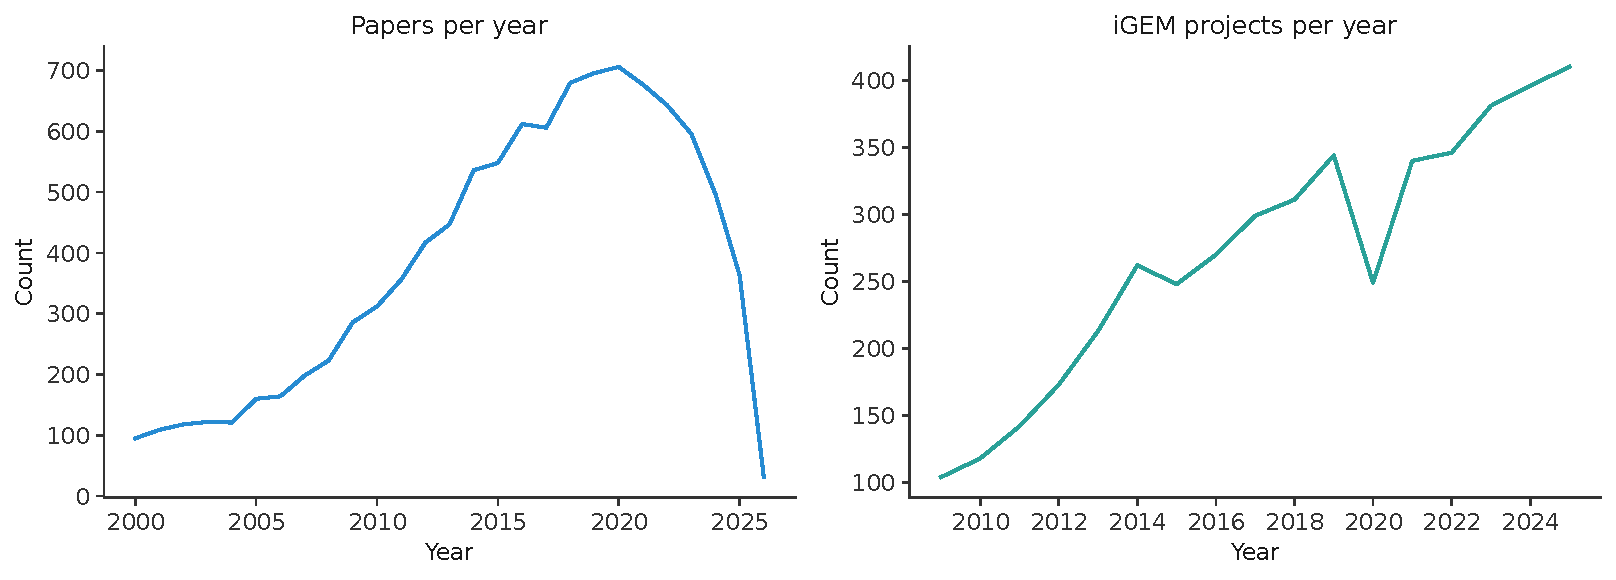
\includegraphics[width=\linewidth]{activity_by_year}
  \caption{Yearly volume of papers (left) and iGEM projects (right). The two
  artifact types cover overlapping but not identical periods, which constrains
  the temporal analysis later in this section.}
  \label{fig:activity}
\end{figure}

% ------------------------------------------------------------
\subsection{Semantic Embeddings}
% ------------------------------------------------------------

To compare text empirically, we need to turn each document into something we can
measure distances between. We do this by building a \textit{semantic embedding
space}: a high-dimensional space in which every document becomes a point, and in
which documents about similar things land close together.

We generate these points with SPECTER2, a natural language model from the Allen
Institute and the successor to the original SPECTER
\citep{cohanDocumentlevelRepresentation2020}.\footnote{SPECTER2 model and
``proximity'' adapter: \url{https://huggingface.co/allenai/specter2}.} SPECTER
belongs to the BERT family of language models \citep{devlinBERTPretrainingDeep2019},
but unlike a general-purpose model it was trained specifically on scientific
papers and their citation graph: it learns to place two documents close together
exactly when one is likely to cite the other. That makes it a natural fit for
our task, where ``related'' is precisely the quantity we are trying to capture.
Each document becomes a 768-dimensional vector.

We chose embeddings over the two obvious alternatives, keyword overlap and
citations, for the same reason. Keyword counting is fragile in synthetic
biology, whose vocabulary overlaps heavily with descriptive molecular biology
\citep{oldhamSyntheticBiologyMapping2018}, so two documents can share words
without sharing meaning, or share meaning while using different words. Citations,
meanwhile, barely exist for student projects. Embeddings sidestep both problems
by working from meaning rather than surface form.

Because SPECTER2 returns unit-length vectors, the natural measure of relatedness
between two documents is the cosine of the angle between them: the closer two
documents point in the same direction, the more semantically related they are.
We use this cosine similarity as the building block for every measure below.

% ------------------------------------------------------------
\subsection{Representing Cities as Centroids}
% ------------------------------------------------------------

A city is not a single document but a cloud of them. To compare cities, we
summarise each cloud by its \textbf{centroid} --- the average of all its
document vectors, re-scaled back to unit length. A city therefore gets two
centroids, one for its papers and one for its projects, each a coarse-grained
``centre of mass'' of that city's work in semantic space.

We then define a city's \textbf{semantic overlap} as the cosine similarity
between its paper centroid and its project centroid. Averaging first and
comparing afterwards is not only faster than comparing every paper to every
project; for unit-length vectors it gives the same answer as the average of all
those pairwise comparisons, which is why centroid-based similarity is a standard
shortcut (Turney \& Pantel, 2010). The idea of summarising a place by the
position of its activity, and reading relatedness off how those positions line
up, follows a long line of work on regional capabilities and the product space
\citep{hidalgoProductSpaceConditions2007, boschmaScientificKnowledgeDynamics2014}.

Figure~\ref{fig:overlap} shows how this measure is distributed across our
\statNCitiesAnalyzed{} cities. Overlap is high and left-skewed, with a mean of
\statOverlapMean{} and a median of \statOverlapMedian{}: most cities sit very
close to 1.0, with a thin tail of low-overlap cities pulling the average down.
The QQ plot confirms the departure from normality (skewness
\statOverlapSkew{}), which matters for any later modelling that assumes
well-behaved errors. Table~\ref{tab:summary} reports the full summary
statistics, and Table~\ref{tab:top15} lists the highest-overlap cities --- all
large, established research hubs with long iGEM histories.

\begin{figure}[htbp]
  \centering
  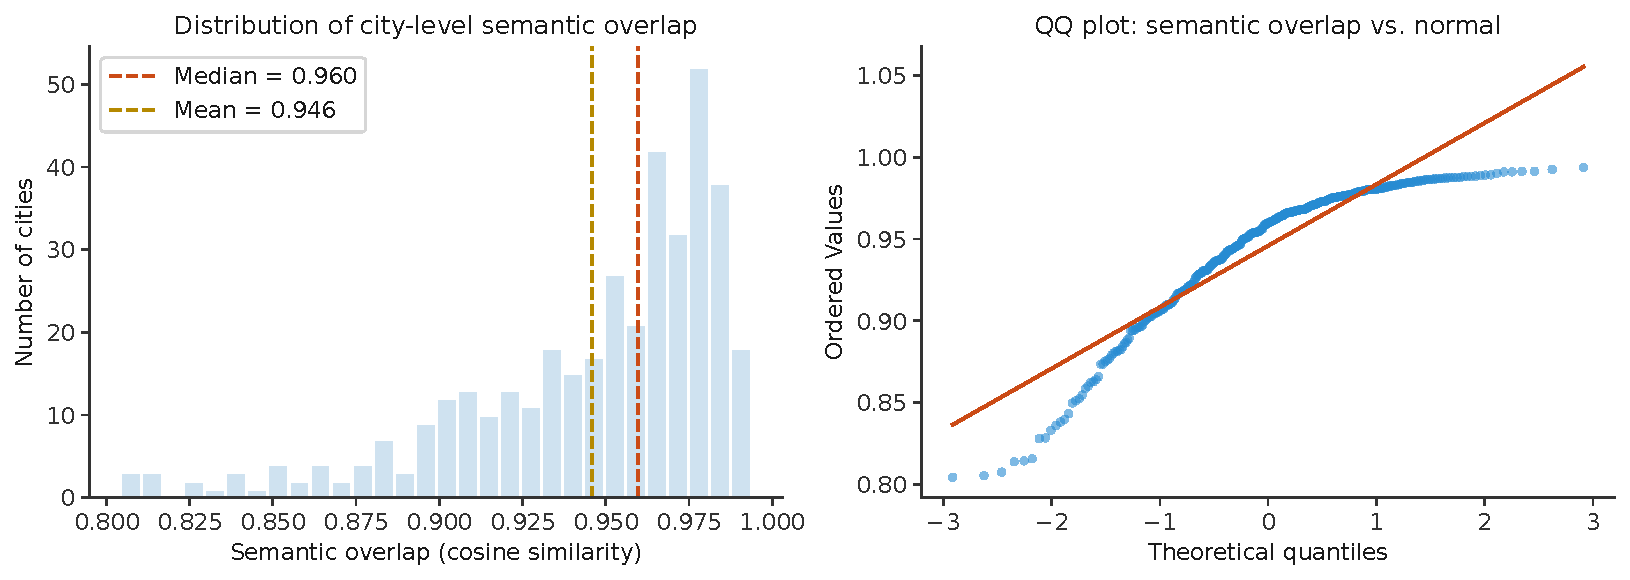
\includegraphics[width=\linewidth]{overlap_distribution}
  \caption{Distribution of city-level semantic overlap (left) and a QQ plot
  against the normal distribution (right). Overlap clusters near 1.0 because all
  documents belong to the same broad field; the spread that remains is what the
  rest of the analysis tries to explain.}
  \label{fig:overlap}
\end{figure}

% Auto-generated by scripts/export_paper_assets.py — do not edit by hand.
\begin{table}[htbp]
\centering
\caption{Summary statistics for the city-level dataset.}
\label{tab:summary}
\begin{tabular}{lrrrrrr}
\toprule
statistic & semantic\_overlap & n\_papers & n\_projects & cs\_paper\_share & cs\_project\_share & proj\_year\_span \\
\midrule
count & 387.000 & 387.000 & 387.000 & 387.000 & 387.000 & 387.000 \\
mean & 0.946 & 20.850 & 9.928 & 0.034 & 0.042 & 7.049 \\
std & 0.040 & 36.471 & 20.626 & 0.103 & 0.126 & 5.749 \\
min & 0.804 & 1.000 & 1.000 & 0.000 & 0.000 & 0.000 \\
25\% & 0.926 & 4.000 & 2.000 & 0.000 & 0.000 & 1.000 \\
50\% & 0.960 & 10.000 & 5.000 & 0.000 & 0.000 & 7.000 \\
75\% & 0.976 & 22.000 & 11.000 & 0.022 & 0.000 & 12.000 \\
max & 0.994 & 364.000 & 258.000 & 1.000 & 1.000 & 16.000 \\
\bottomrule
\end{tabular}

\end{table}

% Auto-generated by scripts/export_paper_assets.py — do not edit by hand.
\begin{table}[htbp]
\centering
\caption{Top 15 cities by semantic overlap.}
\label{tab:top15}
\begin{tabular}{llrrr}
\toprule
city & country & n\_papers & n\_projects & semantic\_overlap \\
\midrule
Cambridge & US & 364 & 40 & 0.994 \\
Shanghai & CN & 126 & 216 & 0.993 \\
Tianjin & CN & 112 & 35 & 0.991 \\
Berkeley & US & 98 & 13 & 0.991 \\
Beijing & CN & 356 & 258 & 0.991 \\
Boston & US & 95 & 25 & 0.991 \\
Hangzhou & CN & 60 & 45 & 0.990 \\
Wuhan & CN & 64 & 102 & 0.989 \\
Changsha & CN & 22 & 26 & 0.989 \\
Urbana & US & 60 & 16 & 0.989 \\
Marburg & DE & 32 & 11 & 0.989 \\
Munich & DE & 58 & 18 & 0.988 \\
Paris & FR & 147 & 37 & 0.988 \\
Guangzhou & CN & 63 & 52 & 0.988 \\
Xiamen & CN & 11 & 21 & 0.988 \\
\bottomrule
\end{tabular}

\end{table}

That high baseline is also a warning. Because every document in the corpus is
synthetic biology, any two city centroids start out fairly close simply by
belonging to the same field, and larger cities --- with more documents averaged
into each centroid --- tend to have steadier, more representative centres.
Figure~\ref{fig:size} makes this concrete: semantic overlap rises with the
number of papers ($r = \statSizePapersR{}$) and projects
($r = \statSizeProjectsR{}$) a city has. This is the familiar tension between
diversity and relatedness in regional science, and it means we cannot read raw
overlap as evidence of local idea flow on its own. The measures that follow are
designed to look past this baseline.

\begin{figure}[htbp]
  \centering
  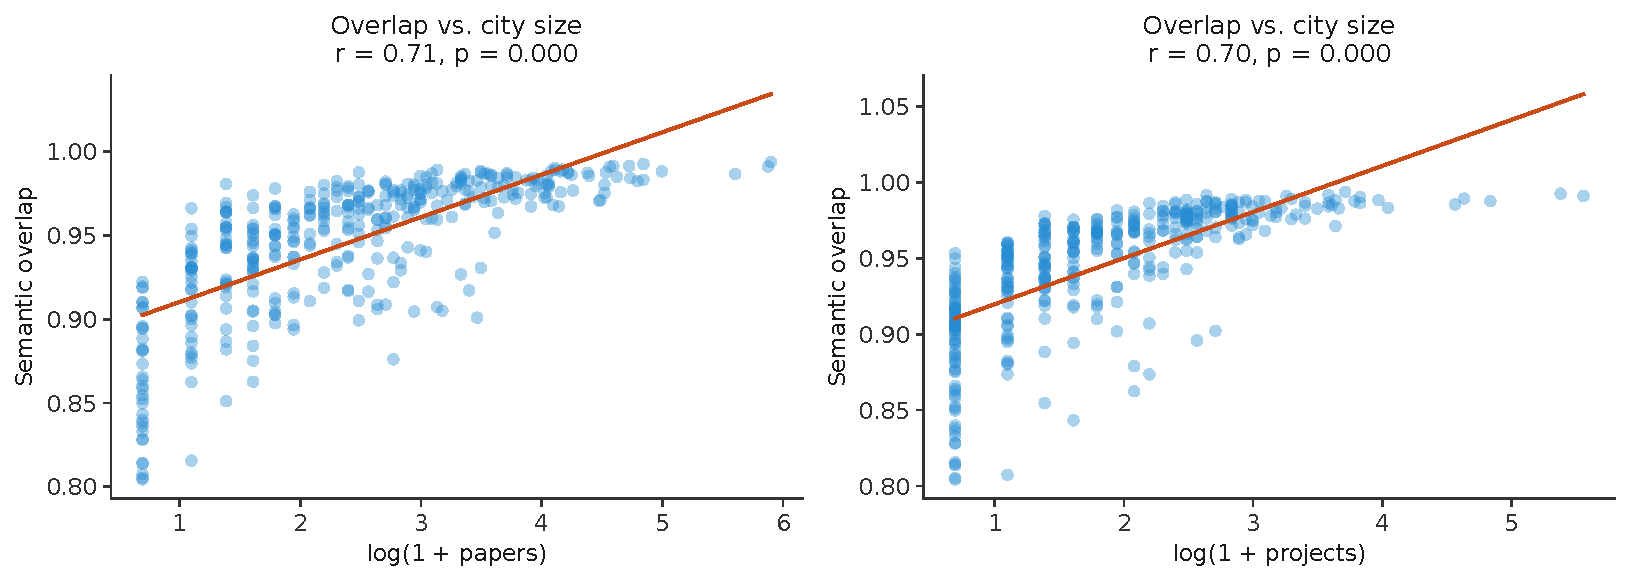
\includegraphics[width=\linewidth]{overlap_vs_size}
  \caption{Semantic overlap against city size, measured by paper count (left)
  and project count (right) on a log scale. Both relationships are strongly
  positive, so part of a city's overlap reflects how much it produces rather
  than how aligned its two outputs are.}
  \label{fig:size}
\end{figure}

% ------------------------------------------------------------
\subsection{Beyond Centroids: Do Projects and Papers Share the Same Topics?}
% ------------------------------------------------------------

The centroid measure has a ceiling we have just seen: because every document is
synthetic biology, two city centroids start close by default, and the spread that
survives is thin and entangled with city size. A sharper question sidesteps the
average altogether. Instead of asking how nearly two centroids point in the same
direction, we ask \textit{which specific topics} a city works on, and whether its
students and its scholars work on the \textit{same} ones.

To do that we first sort the documents into topics. We run HDBSCAN --- a
density-based clustering algorithm that finds dense groups without our having to fix
their number in advance, and sets aside documents too sparse to belong as ``noise''
(Campello, Moulavi \& Sander, 2013) --- over the embedding space, which yields a few
hundred coherent sub-themes (biosensors, metabolic engineering, genome assembly, and
the like). Each city then gets two \textit{cluster-frequency vectors}: the share of
its papers that fall in each topic, and the share of its projects. We define a
city's \textbf{cluster co-membership} as the cosine between those two vectors. Unlike
the centroid overlap, this number is high \textit{only} when papers and projects
occupy the same specific topics, and near zero when they occupy different ones: the
field-level baseline cancels, because belonging to synthetic biology is no longer
enough to score.

That sharpness costs data. With several hundred topics, a city holding only a
handful of documents can miss its own themes by chance, leaving its two vectors
looking unrelated for want of observations rather than for want of relatedness. We
therefore compute the measure only for cities with at least \statClusterMinDocs{}
clustered documents of each type --- \statClusterNCitiesDense{} of the
\statClusterNCitiesAll{} cities that have any clustered work of both kinds. A sweep
across thresholds confirms this is a measurement floor and not a finding: below it
most cities score exactly zero, while above it a signal emerges and strengthens as
the threshold rises.

We then subject the measure to the test the centroid overlap could not pass. We ask
whether a city's own papers and own projects share topics by more than chance with a
\textbf{re-pairing permutation test}: within each country we randomly reassign which
city's project-vector is matched against which city's paper-vector, recompute the
average co-membership, and repeat two thousand times (Good, 2005). This null keeps
each country's mix of work intact while destroying the local pairing, so it isolates
exactly the quantity at issue --- whether a city's two outputs are aligned beyond
what a same-country neighbour would supply. The observed mean co-membership is
\statClusterPermObserved{}, against a null mean of \statClusterPermNullMean{}
(permutation $p = \statClusterPermP{}$; an excess of \statClusterPermExcess{}, about
half again above chance). And unlike raw overlap, it is not a size effect: regressed
on the log counts of a city's papers and projects it leaves only
$R^2 = \statClusterOlsRsq{}$, with neither coefficient reaching significance
($p = \statClusterSizePapersP{}$ and $\statClusterSizeProjectsP{}$).
Figure~\ref{fig:cluster} shows the contrast with the centroid measure alongside the
permutation null.

\begin{figure}[htbp]
  \centering
  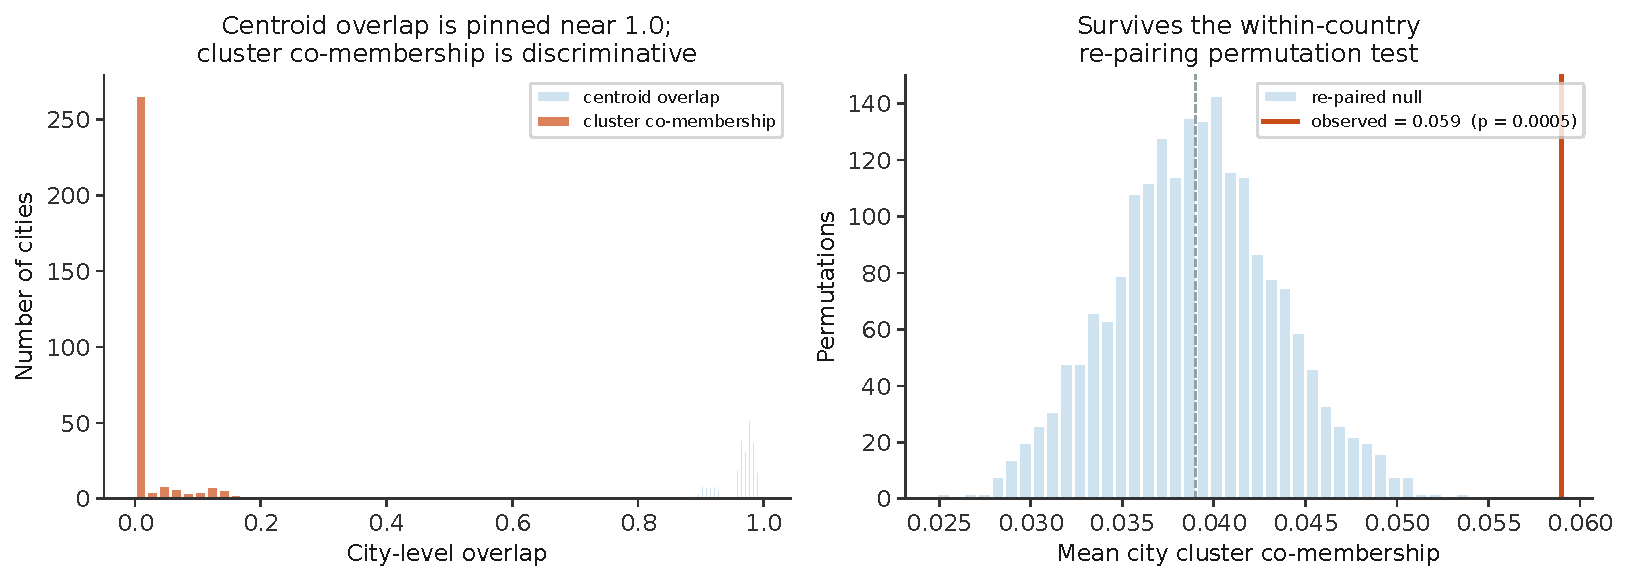
\includegraphics[width=\linewidth]{cluster_comembership}
  \caption{Cluster co-membership. Left: the distribution of the centroid overlap
  (pinned near 1.0 by the shared field) against cluster co-membership, which spreads
  out because it scores only shared \textit{specific} topics. Right: the
  within-country re-pairing permutation null for the mean co-membership across cities
  with at least \statClusterMinDocs{} documents of each type; the observed value sits
  far into the right tail ($p = \statClusterPermP{}$), passing the test the centroid
  measure fails.}
  \label{fig:cluster}
\end{figure}

% ------------------------------------------------------------
\subsection{Local Alignment: Is a Project Closer to Its Own City?}
% ------------------------------------------------------------

Instead of comparing the two centroids of a single city, we can ask a sharper
question one project at a time: is an individual iGEM project more similar to its
\textit{own} city's papers than to the papers of every other city? If projects
and papers really share local roots, the answer should be yes.

For each project we compute its cosine similarity to its home city's paper
centroid, and its average similarity to the paper centroids of all other cities
(keeping only cities with at least three papers, so the centroids are stable).
The difference between the two, which we call $\delta$, is positive whenever a
project looks more like home than like elsewhere. Across \statAlignNProjects{}
projects the mean advantage is $\delta = \statAlignMeanDelta{}$, and
\statAlignFracPos{} of projects are individually positive.
Figure~\ref{fig:align} shows the full distribution and the project-by-project
comparison.

A word on how we count, because it changes the headline number. Projects from
the same city are all compared against the \textit{same} paper centroid, so they
are not independent observations; a naive one-sample test
($t = \statAlignT{}$) badly overstates its confidence by treating
\statAlignNProjects{} correlated projects as if they were that many independent
draws. The honest unit of analysis is the city. Clustering the standard error at
the city level --- the intercept-only case of the standard cluster-robust
estimator (Cameron \& Miller, 2015) --- brings the statistic down to
$t = \statAlignTClustered{}$ across \statAlignNCities{} cities, and aggregating
to a single mean $\delta$ per city before testing tells the same story
($\delta = \statAlignDeltaCity{}$, $t = \statAlignTCity{}$, with
\statAlignFracCitiesPos{} of cities on the home-city side). The effect is small in
absolute terms --- a consequence of the field-level baseline noted above --- but
it is real and it survives being counted properly. We read it as evidence of
local \textit{relatedness}, not of any causal pull, since a shared university
faculty could easily produce both kinds of work on the same theme without one
feeding the other.

\begin{figure}[htbp]
  \centering
  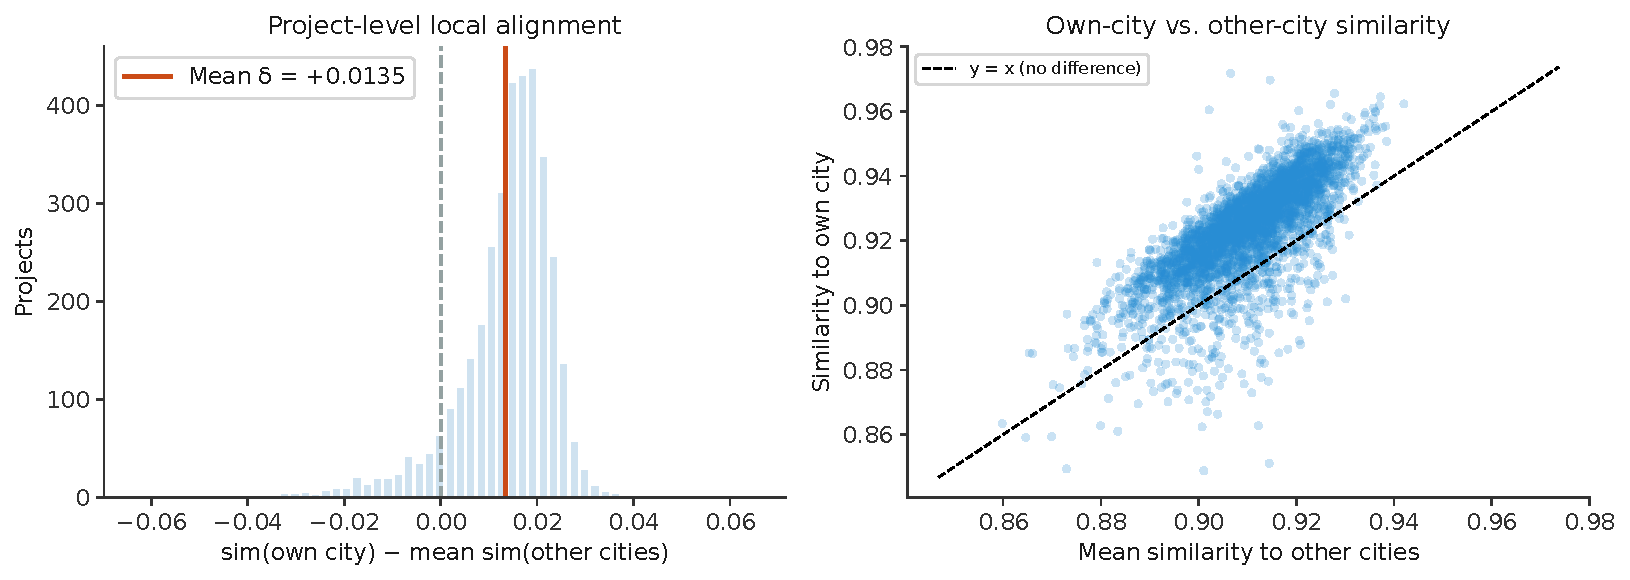
\includegraphics[width=\linewidth]{project_level_alignment}
  \caption{Local alignment at the project level. Left: the distribution of
  $\delta$, each project's similarity to its own city's papers minus its mean
  similarity to other cities' papers; mass to the right of zero indicates local
  alignment. Right: own-city versus other-city similarity, where points above
  the diagonal are the locally aligned projects.}
  \label{fig:align}
\end{figure}

% ------------------------------------------------------------
\subsection{Stable Specialisation versus Local Timing: A Difference-in-Differences Design}
% ------------------------------------------------------------

The local advantage in the previous test could mean two quite different things.
It might reflect a genuine, time-specific connection --- this year's projects
tracking this year's local papers. Or it might just reflect a city's stable
identity: a place that has always worked on biosensors will have both projects
and papers about biosensors in every year, with no idea flowing between them at
all. To separate these, we borrow the logic of a \textbf{difference-in-differences}
design, the workhorse of applied econometrics (Angrist \& Pischke, 2009).

The idea is a two-by-two comparison. For each project we measure its similarity
to its own city's papers and to other cities' papers, and we do this both in the
project's \textit{own year} and in \textit{other years}. A stable-specialisation
story predicts a home-city advantage even in other years; a local-timing story
predicts an \textit{extra} advantage in the project's own year, on top of that.
The difference-in-differences is exactly that extra slice. Table~\ref{tab:did}
reports the four cells, and Figure~\ref{fig:did} shows them alongside the
distribution of the per-project estimate.

% Auto-generated by scripts/export_paper_assets.py — do not edit by hand.
\begin{table}[htbp]
\centering
\caption{Difference-in-differences cells: mean cosine similarity between iGEM projects and annual paper centroids.}
\label{tab:did}
\begin{tabular}{lrr}
\toprule
 & Own city & Other cities \\
\midrule
Own year & 0.9125 & 0.8990 \\
Other years & 0.9063 & 0.8954 \\
\bottomrule
\end{tabular}

\end{table}

Across \statDidN{} projects the estimate is positive and survives the same
city-level clustering used above ($\text{DiD} = \statDidEstimate{}$,
$t = \statDidTClustered{}$ clustered across \statDidNCities{} cities; the naive
$t = \statDidT{}$ again overstates the precision), but it is tiny next to the
stable-specialisation gap that sits underneath it. In plain terms: most of why a
project resembles its city's papers is that the city has a durable thematic
identity, with only a sliver attributable to same-year alignment. This is a
useful corrective to a naive reading of the local-alignment result, and we return
to it as the analytical centrepiece of the Results.

\begin{figure}[htbp]
  \centering
  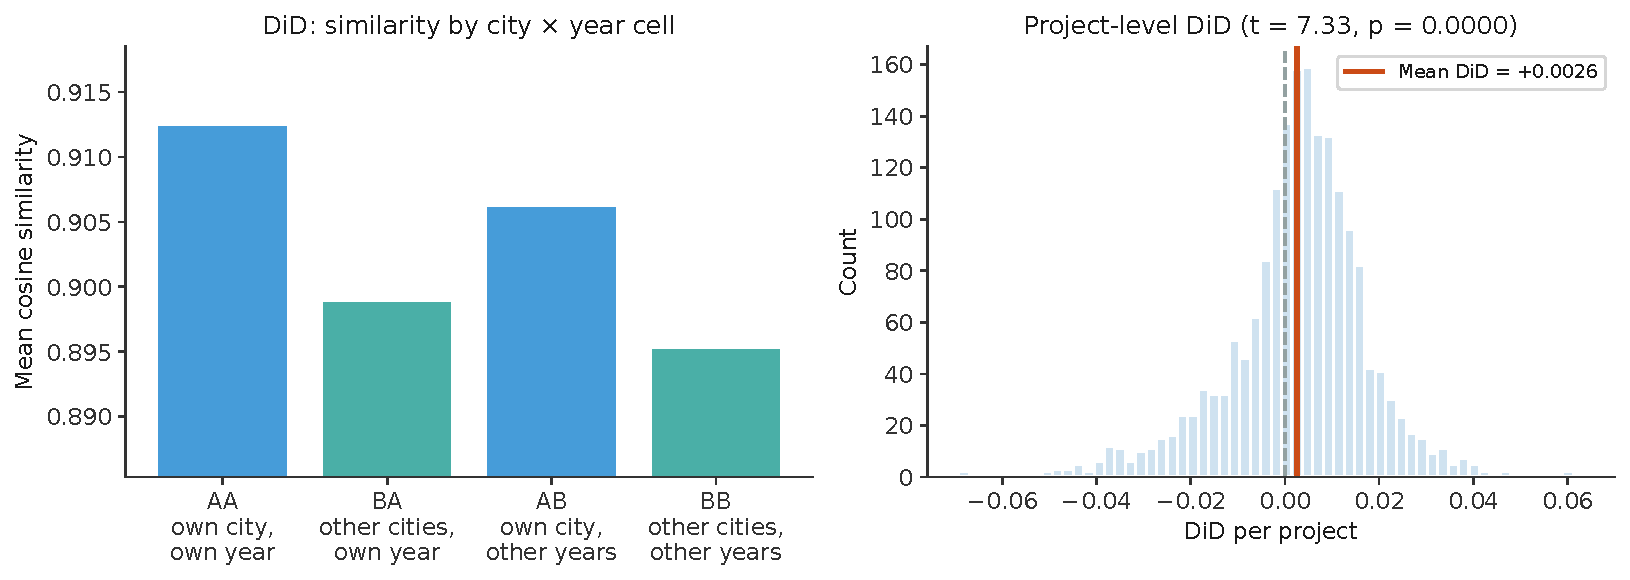
\includegraphics[width=\linewidth]{did_alignment}
  \caption{Difference-in-differences. Left: mean similarity in each of the four
  city\,$\times$\,year cells. Right: the distribution of the per-project
  difference-in-differences; its small positive mean is the part of local
  alignment that is specific to the project's own year.}
  \label{fig:did}
\end{figure}

% ------------------------------------------------------------
\subsection{Temporal Structure: Do Projects Lead Papers?}
% ------------------------------------------------------------

The guiding intuition of this thesis is that student projects might introduce
early ideas that academic papers later develop. If so, a city's projects in year
$t$ should look most like its papers a few years \textit{after} $t$. To test the
shape of this relationship we build annual centroids for each city's projects and
papers, and for every project-year we record its similarity to the city's paper
centroid at offsets from three years before to three years after. Averaging over
all city-years gives a \textbf{lead--lag profile}: similarity as a function of
the offset $k$, where positive $k$ means papers come after projects. This is the
descriptive, correlational cousin of a Granger lead--lag analysis (Granger,
1969); we use it to describe timing, not to claim causation.

Figure~\ref{fig:leadlag} and Table~\ref{tab:leadlag} show the result, and the
honest summary is that the profile is nearly flat. The nominal peak sits at
$k = \statLeadlagBestLag{}$ (mean similarity \statLeadlagBestSim{}), which would
be consistent with projects leading papers, but the difference across the whole
range is on the order of a thousandth of a cosine unit and the confidence
intervals overlap almost everywhere. Our reading is that city-level annual
centroids are simply too coarse --- often built from a single document in a given
year --- to resolve a lead--lag signal if one exists. We report the test because
the null result is informative about the method, not because it settles the
question.

% Auto-generated by scripts/export_paper_assets.py — do not edit by hand.
\begin{table}[htbp]
\centering
\caption{Lead-lag similarity profile between project and paper centroids.}
\label{tab:leadlag}
\begin{tabular}{rrrrr}
\toprule
lag & n\_pairs & mean\_sim & ci\_lo & ci\_hi \\
\midrule
-3 & 1253 & 0.8950 & 0.8927 & 0.8972 \\
-2 & 1300 & 0.8966 & 0.8946 & 0.8988 \\
-1 & 1357 & 0.8975 & 0.8952 & 0.8997 \\
0 & 1383 & 0.8988 & 0.8966 & 0.9008 \\
1 & 1324 & 0.9000 & 0.8979 & 0.9020 \\
2 & 1270 & 0.8997 & 0.8975 & 0.9019 \\
3 & 1189 & 0.9003 & 0.8981 & 0.9025 \\
\bottomrule
\end{tabular}

\end{table}

\begin{figure}[htbp]
  \centering
  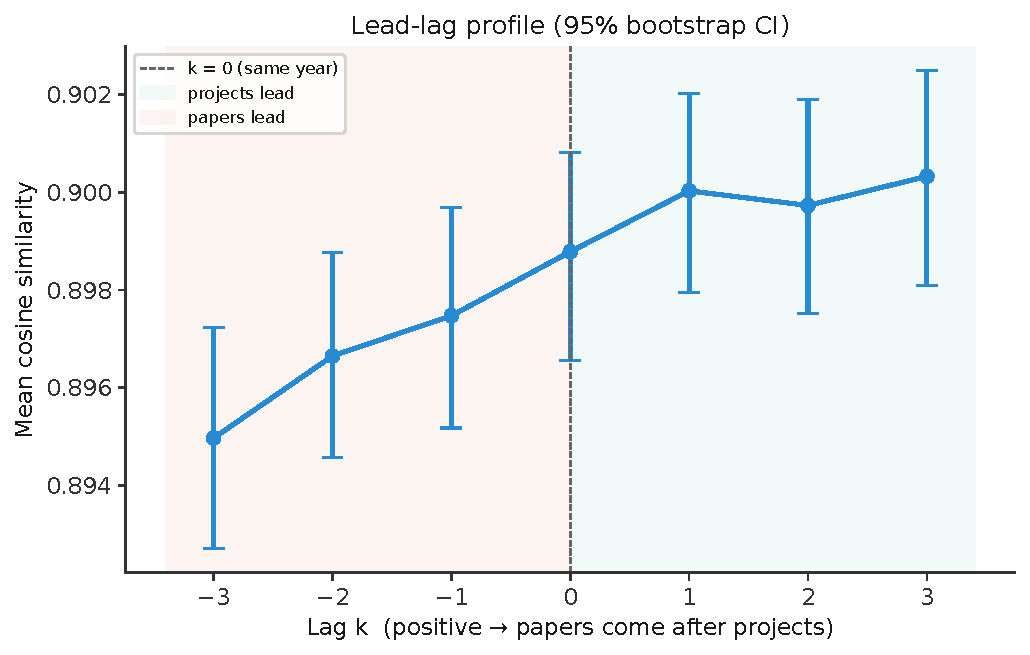
\includegraphics[width=0.72\linewidth]{lead_lag_profile}
  \caption{Lead--lag profile between project and paper centroids, with 95\%
  bootstrap confidence intervals. Positive lags mean papers follow projects. The
  profile is close to flat, so the data neither confirm nor rule out the
  early-signal hypothesis.}
  \label{fig:leadlag}
\end{figure}

% ------------------------------------------------------------
\subsection{Beyond Text: BioBrick Part-Type Composition}
% ------------------------------------------------------------

Everything so far rests on text. As an independent check, we turn to the
physical parts each city's teams actually registered. The \textit{mix} of part
types a city deposits --- coding sequences, regulatory elements, reporters, and
so on --- is a fingerprint of the kind of biology it does, and it is measured
completely separately from the embedding space. If our text-based picture is
capturing something real, the two should broadly agree.

For each city with at least ten registered parts (\statNCitiesParts{} cities in
all) we compute the share of its parts in each functional category, and summarise
how specialised that mix is with its Shannon entropy: low entropy means a city
concentrates on one type of part, high entropy means it spreads across many. The
median city sits at \statPartEntropyMedian{} nats, well below the
\statPartEntropyMax{} nats a perfectly even spread would give, so cities do tend
to specialise. Figure~\ref{fig:parts} shows the spread of specialisation and the
part-type fingerprints of the most active cities.

\begin{figure}[htbp]
  \centering
  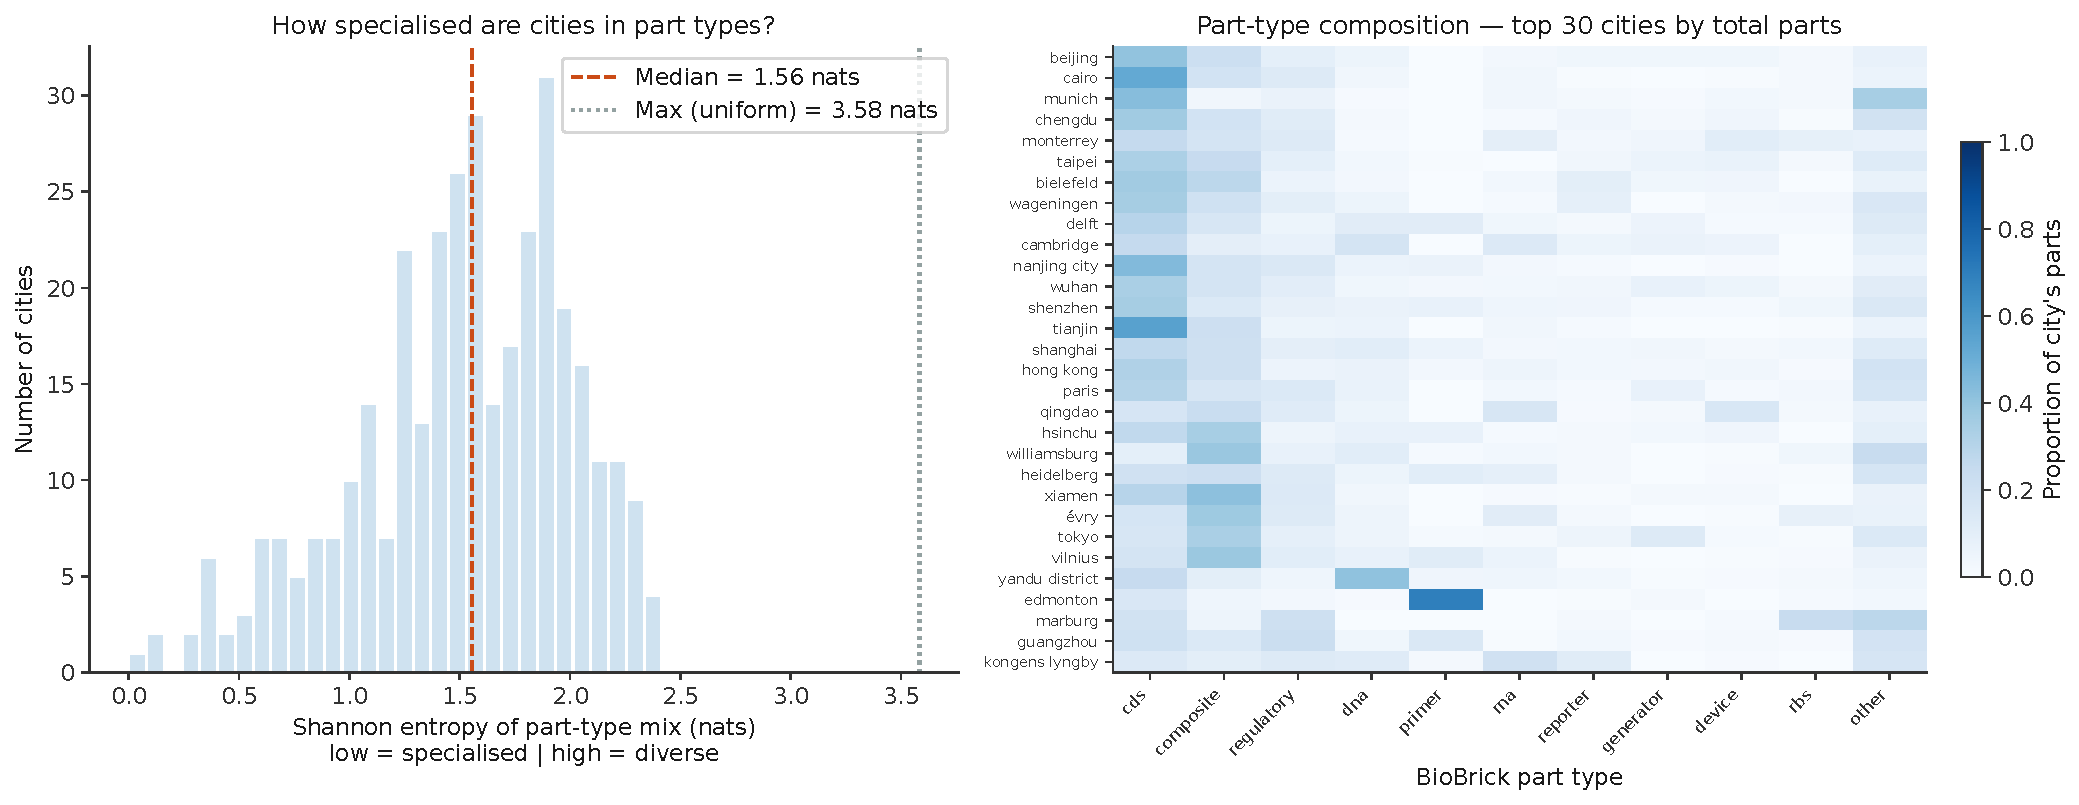
\includegraphics[width=\linewidth]{part_type_composition}
  \caption{BioBrick part-type composition. Left: the distribution of part-type
  entropy across cities; most cities lean toward specialisation. Right: the
  part-type profile of the thirty cities with the most registered parts, sorted
  so that cities with a shared dominant type sit together.}
  \label{fig:parts}
\end{figure}

% ------------------------------------------------------------
\subsection{Interpretive Caution}
% ------------------------------------------------------------

Two limitations shape how far these measures can be pushed, and we flag them here
rather than burying them. First, because the entire corpus is synthetic biology,
cosine similarity between city centroids is dominated by field-level similarity:
two cities look alike mostly because they both do synthetic biology, and only
secondarily because of any genuine local alignment. The difference-in-differences
result makes this concrete, and it is why we lean on the sharper, within-city
comparisons rather than on raw overlap. The sharpest of those, cluster
co-membership, carries its own caveat in turn: it can only be computed where a city
has enough documents to estimate a topic distribution, so its permutation result
speaks to the \statClusterNCitiesDense{} most active cities rather than to the long
tail. Second, papers are geocoded to a single
affiliation, so multi-city collaborations are flattened, and our annual centroids
are too thin to support fine temporal claims. Accordingly we frame every result
in this section as semantic relatedness and plausible co-location, and we leave
claims of causal knowledge flow to future work with finer, author- and
mentor-level data.

% ============================================================
\section{Results}
% ============================================================

The Methods section reported each measure's numbers where it built the measure.
Here we step back and read those numbers as a sequence of escalating claims, each
more demanding than the last. The first is a sanity check: that the embedding space
recovers a recognisable map of the field at all. The second is the thesis's central
empirical claim: that a city's student projects and its academic papers occupy the
\textit{same specific topics}, not merely the same broad field --- a local
relatedness that, measured by cluster co-membership, survives a permutation test the
raw centroid overlap cannot. A project-level alignment test corroborates it from a
second direction, and decomposing that alignment shows how much is live, same-year
coupling (little) versus standing thematic identity (most). The third claim is the
most ambitious, and the one we can least support: that the two are linked in time,
with projects running ahead of papers. We take them in turn, then ask whether
anything outside the text agrees.

% ------------------------------------------------------------
\subsection{The Embedding Space Recovers a Sensible Map}
% ------------------------------------------------------------

Before asking whether projects and papers align, we should check that the space
they live in is meaningful. Two features suggest it is. The cities with the
highest project--paper overlap (Table~\ref{tab:top15}) are precisely the places
one would name without any model in hand: Cambridge, Boston and Berkeley in the
United States; Beijing, Shanghai, Tianjin and Wuhan in China; Munich and Marburg
in Germany; Paris in France --- large, long-running synthetic biology hubs with
deep iGEM histories. The cities at the other end (Table~\ref{tab:bottom15}) are
almost all places with a single paper and a single project, where a centroid is
just one document and overlap is whatever that lone pairing happens to be. Low
overlap, in other words, tracks thin data rather than genuine thematic
divergence, exactly as the size relationship ($r = \statSizePapersR{}$ for
papers, $r = \statSizeProjectsR{}$ for projects) leads us to expect. The map
behaves the way a sensible map should: it puts the well-known hubs at the top and
reserves its uncertainty for the cities we know least about.

% Auto-generated by scripts/export_paper_assets.py — do not edit by hand.
\begin{table}[htbp]
\centering
\caption{Bottom 15 cities by semantic overlap.}
\label{tab:bottom15}
\begin{tabular}{llrrr}
\toprule
city & country & n\_papers & n\_projects & semantic\_overlap \\
\midrule
Guwahati & IN & 3 & 1 & 0.851 \\
Santa Clara & US & 1 & 1 & 0.850 \\
Roorkee & IN & 1 & 4 & 0.843 \\
Noda & JP & 1 & 1 & 0.840 \\
Phoenix & US & 1 & 1 & 0.838 \\
Bogor & ID & 1 & 1 & 0.836 \\
Agra & IN & 1 & 1 & 0.833 \\
Merced & US & 1 & 1 & 0.828 \\
León & ES & 1 & 1 & 0.828 \\
Tampa & US & 2 & 1 & 0.816 \\
West Point & US & 1 & 1 & 0.814 \\
Orléans & FR & 1 & 1 & 0.814 \\
Kfar Saba & IL & 1 & 2 & 0.807 \\
Charleston & US & 1 & 1 & 0.805 \\
Boca Raton & US & 1 & 1 & 0.804 \\
\bottomrule
\end{tabular}

\end{table}

% ------------------------------------------------------------
\subsection{A City's Projects and Papers Share Its Specific Topics}
% ------------------------------------------------------------

The central finding is that a city's student projects and its academic papers
concentrate in the \textit{same specific corners} of synthetic biology, not just the
same broad field. Measured as cluster co-membership --- the cosine between a city's
paper and project topic-distributions --- the average city, among the
\statClusterNCitiesDense{} with enough documents to measure it, scores
\statClusterPermObserved{}, well above the \statClusterPermNullMean{} expected when
we re-pair papers and projects across same-country cities at random (permutation
$p = \statClusterPermP{}$). In plain terms: a city's two kinds of output land in the
same topics far more often than a comparable neighbour's would, and the gap is large
relative to chance --- an excess of \statClusterPermExcess{}, roughly half again
above the null.

What makes this the result the draft leans on, rather than the raw centroid overlap,
is that it clears two bars the centroid measure cannot. It is not an artifact of the
field baseline: by scoring only shared \textit{specific} topics, it starts from zero
for unrelated cities rather than from the near-1.0 floor every synthetic-biology
centroid sits on. And it is not an artifact of city size: the same kind of regression
that explains most of the centroid overlap explains almost none of this measure
($R^2 = \statClusterOlsRsq{}$, with neither size coefficient significant), so we are
not merely rediscovering that large cities have steadier centres. A measure built to
survive both objections does survive them, which is why we read its permutation
result as the thesis's strongest evidence of genuine local relatedness.

% ------------------------------------------------------------
\subsection{Projects and Papers Co-specialise Within Cities}
% ------------------------------------------------------------

A second line of evidence works one project at a time: an iGEM project sits closer
to its own city's papers than to other cities' papers. The raw advantage is small but pervasive ---
$\delta = \statAlignMeanDelta{}$, with \statAlignFracPos{} of projects on the
home-city side --- and, crucially, it holds up once we count cities rather than
projects. Clustered at the city level the advantage stands at
$t = \statAlignTClustered{}$ across \statAlignNCities{} cities, and
\statAlignFracCitiesPos{} of cities (not just projects) lean toward home.
Whatever else is true, a city's student work really does resemble its own
academic work more than a stranger's.

But ``closer to home'' can mean two very different things, and separating them is
the analytical heart of this draft. The home-city advantage might be a
\textit{timing} signal --- this year's projects tracking this year's local
papers, the kind of live coupling a knowledge pipeline would produce --- or it
might be pure \textit{stable specialisation}: a city that has always done
biosensors will show biosensor projects and biosensor papers in every year, with
no ideas passing between them. The difference-in-differences design isolates the
timing slice from the standing one (Table~\ref{tab:did}). The verdict is sobering
for the pipeline story: of the whole home-city advantage, only \statDidEstimate{}
is specific to a project's own year ($t = \statDidTClustered{}$ clustered across
\statDidNCities{} cities --- small, but really there), while the rest is a
durable thematic identity that holds across years. Co-specialisation is real, but
it is mostly something a city \textit{is}, not something that \textit{happens}
between its students and its scholars in a given year. This is a more modest claim
than a knowledge pipeline, and it is the one the data actually support.

That co-specialisation is also unevenly distributed, in a way that is itself
informative. The home-city advantage grows with the size of a city's research
base: across cities, mean $\delta$ rises with the (log) number of local papers
($r = \statAlignSizeR{}$), and projects in above-median cities enjoy more than
three times the advantage of those in the long tail ($\delta =
\statAlignDeltaLarge{}$ versus $\statAlignDeltaSmall{}$). Local alignment, in
other words, is largely a feature of mature clusters --- the Beijings and Bostons
with enough of both kinds of work to have built a coherent local identity --- and
fades, without quite vanishing, in cities with only a project or two. That is a
more useful finding for innovation policy than a flat average would be: it
suggests the project--paper link is something clusters \textit{grow into} as
their research base thickens.

Finally, the carbon-capture case study behaves just like the whole. Restricting
the alignment test to the \statCcAlignN{} carbon-capture projects (across
\statCcAlignNCities{} cities) gives essentially the same picture as the full
corpus --- $\delta = \statCcAlignMeanDelta{}$, \statCcAlignFracPos{} of projects
on the home-city side, $t = \statCcAlignTClustered{}$ clustered by city. The
thread we promised to follow is not an exception: a city's carbon-capture
students sit nearer its own carbon-relevant literature than elsewhere's, exactly
as the general result predicts.

% ------------------------------------------------------------
\subsection{Timing Is Unresolved, but the Parts Agree}
% ------------------------------------------------------------

The most ambitious claim --- that projects lead papers --- we cannot make, and the
reason is worth stating as a result in its own right. The lead--lag profile
(Table~\ref{tab:leadlag}, Figure~\ref{fig:leadlag}) rises gently from lag $-3$ to
lag $+3$, with its nominal peak at $k = \statLeadlagBestLag{}$ years, the
direction the early-signal hypothesis predicts. But the whole profile spans about
a thousandth of a cosine unit and the confidence intervals overlap throughout, so
we treat it as flat. This is best read as a \textit{negative methodological
result}: a centroid averaged over the one or two documents a small city produces
in a given year carries almost no temporal information, so timing simply cannot be
read off centroids at this resolution. Resolving it will take a sharper instrument
--- the project--part--paper citation graph described in the Background, where a
single project's parts point to dated literature directly --- which we flag as the
natural next step rather than a finding of this draft.

What does survive is an independent corroboration from outside the text. The mix
of BioBrick part types a city registers --- measured with no reference to the
embedding space --- shows the same specialisation the text does
(Figure~\ref{fig:parts}): the median city's part-type entropy is
\statPartEntropyMedian{} nats against a possible \statPartEntropyMax{}, so cities
concentrate on particular kinds of biology rather than spreading evenly. More
directly, cities that look alike in part-type space also look alike in
topic-cluster space: correlating the two sets of city-to-city similarities --- a
Mantel test (Mantel, 1967) --- gives a clear positive association across
\statMantelNCities{} cities ($r = \statMantelR{}$, $p = \statMantelP{}$ against a
label-shuffling null), so the physical parts and the abstract text rank the cities
the same way. That two methods built on entirely different data --- abstract text on
one side, registered parts on the other --- both point to local specialisation gives
us more confidence that the specialisation lives in the cities, not in the model.

% ============================================================
\section{Conclusion}
% ============================================================

The question this draft set out to answer was whether cities that host student
synthetic biology projects also produce academic papers in related areas. The
answer is a qualified yes. Its strongest form is topical: in cities active enough to
measure it, a city's projects and papers fall in the \textit{same specific}
sub-fields far more than a same-country neighbour's would (cluster co-membership,
permutation $p = \statClusterPermP{}$), a relatedness that holds up after stripping
out both the field-level baseline and city size. The centroid-based tests tell the
same story from a second angle. A city's iGEM projects sit measurably nearer its own
papers than other cities' papers; the pattern holds across roughly nine of every
ten projects and, more tellingly, across four in five \textit{cities} once the
inference is clustered where it belongs; it is strongest in large, mature research
hubs but still positive in the long tail; it reappears essentially unchanged in
the carbon-capture case study; and it is echoed by a parts-based fingerprint that
never touches the embedding model. Cities do appear to specialise, and their
student and academic work specialises together.

Two qualifications keep that finding honest. First, the alignment is mostly a
stable feature of a city's identity rather than a year-by-year coupling: the
difference-in-differences result shows that the same-year, ``this project tracks
this paper'' component, while statistically real even under city-level
clustering, is small next to the standing thematic gap. We therefore describe a
\textit{local innovation trajectory} as shared standing specialisation, not as a
demonstrated flow of ideas from students to scholars. Second, our strongest
temporal hypothesis --- that projects run ahead of papers --- is neither confirmed
nor refuted; the city--year centroids are too thin to resolve it, and resolving it
will take the finer, graph-level instrument we turn to below. Both qualifications
echo the interpretive caution in the Methods: with a corpus that is entirely
synthetic biology, field-level similarity sets a high baseline, and the signal we
care about lives in the small margins on top of it.

These limits also point the way forward, and mark where the project's remaining
reach --- patents, and the planet-scale application that motivates the whole
effort --- comes in. The clearest gains would come from finer links than centroids
can provide: scraping the DOIs that iGEM teams cite on their wikis, to build a
direct citation network between projects and the local literature; matching paper,
patent, and team authors to ask whether researchers stay in the orbit of their old
iGEM collaborators; and matching BioBrick sequences to patent filings through
sequence databases, to trace individual pieces of genetic code from an open
registry into commercial application. Each would replace a coarse, centroid-level
association with a concrete, traceable link --- and would let a future study ask
not just whether a city's projects and papers are related, but whether one
actually grew out of the other.

\bibliographystyle{plainnat}
\bibliography{references}

\end{document}
